
\documentclass[paper=a4, fontsize=11pt]{scrartcl}		% KOMA article
\usepackage[a4paper,pdftex]{geometry}										% A4paper margins
\setlength{\oddsidemargin}{5mm}												% Remove 'twosided' indentation
\setlength{\evensidemargin}{5mm}


\usepackage[dvipsnames]{xcolor}
\usepackage{fancyvrb}
\usepackage{spverbatim}

% redefine \VerbatimInput
\RecustomVerbatimCommand{\VerbatimInput}{VerbatimInput}%
{fontsize=\footnotesize,
 %
 frame=lines,  % top and bottom rule only
 framesep=2em, % separation between frame and text
 rulecolor=\color{Gray},
 %
 labelposition=topline,
 %
 commandchars=, % escape character and argument delimiters for
                      % commands within the verbatim
 commentchar=*        % comment character
}



\usepackage[english]{babel}
\usepackage[protrusion=true,expansion=true]{microtype}
\usepackage{amsmath,amsfonts,amsthm,amssymb}
\usepackage{graphicx}
\graphicspath{{./figures/}}
\usepackage{caption}
\usepackage{multicol}
\usepackage{cite}
\usepackage{graphicx}
\usepackage{hyperref}
\usepackage{url}
\usepackage{float}
% ------------------------------------------------------------------------------
% Definitions (do not change this)
% ------------------------------------------------------------------------------
\newcommand{\HRule}[1]{\rule{\linewidth}{#1}} 	% Horizontal rule

\makeatletter							% Title
\def\printtitle{%
    {\centering \@title\par}}
\makeatother

\makeatletter							% Author
\def\printauthor{%
    {\centering \large \@author}}
\makeatother

% \setlength\parindent{0pt} % Removes all indentation from paragraphs

%==================================================================================================
% Source Code
%==================================================================================================
\usepackage{listings}
\lstdefinelanguage{JavaScript}{
  keywords={typeof, new, true, false, catch, function, return, null, catch, switch, var, if, in, while, do, else, case, break},
  keywordstyle=\color{blue}\bfseries,
  ndkeywords={class, export, boolean, throw, implements, import, this},
  ndkeywordstyle=\color{darkgray}\bfseries,
  identifierstyle=\color{black},
  sensitive=false,
  comment=[l]{//},
  morecomment=[s]{/*}{*/},
  commentstyle=\color{purple}\ttfamily,
  stringstyle=\color{red}\ttfamily,
  morestring=[b]',
  morestring=[b]"
}
% \usepackage{xcolor}
\definecolor{mygray}{gray}{0.3}
\definecolor{darkgreen}{RGB}{0,127,0}
\definecolor{darkred}{RGB}{180,0,0}
\definecolor{mygray2}{gray}{0.9}
\definecolor{darkgreen}{RGB}{0,127,0}
\definecolor{darkred}{RGB}{180,0,0}
\definecolor{mygray2}{gray}{0.9}

% \usepackage[scaled]{beramono} % Bera Mono font
\lstset{
  basicstyle=\footnotesize, % Standardschrift
  %numbers=left,              % Ort der Zeilennummern
  numberstyle=\tiny,          % Stil der Zeilennummern
  %stepnumber=2,              % Abstand zwischen den Zeilennummern
  numbersep=5pt,              % Abstand der Nummern zum Text
  tabsize=2,                  % Groesse von Tabs
  extendedchars=false,
  %texcl=true,
  %escapechar=\$,
  breaklines=true,            % Zeilen werden Umgebrochen
  keywordstyle=\color{blue},
  frame=b,
  identifierstyle=\color{darkred},
  commentstyle=\color{mygreen},%\textit,
  showspaces=false,           % Leerzeichen anzeigen ?
  showtabs=false,             % Tabs anzeigen ?
  xleftmargin=17pt,
  framexleftmargin=17pt,
  framexrightmargin=5pt,
  framexbottommargin=4pt,
  escapeinside={\%*}{*)},
  stringstyle=\color{mymauve},
  %backgroundcolor=\color{lightgray},
  showstringspaces=false      % Leerzeichen in Strings anzeigen ?
  %,classoffset=1,
  %morekeywords={1,2,3,4,5,6,7,8,9,0},
  %keywordstyle=\color{yellow},
  %classoffset=0
}

\DeclareCaptionFont{white}{\color{white}}
\DeclareCaptionFormat{listing}{\colorbox[cmyk]{0.43, 0.35, 0.35,0.01}{\fontfamily{phv}\selectfont\parbox{\textwidth}{\hspace{15pt}#1#2#3}}}
\captionsetup[lstlisting]{
  format          = listing,
  labelfont       = white,
  textfont        = white,
  singlelinecheck = false,
  margin          = 0pt,
  font            = {bf,footnotesize}
}
\usepackage{framed}

\usepackage{caption}
\captionsetup[lstlisting]{font={small,tt}}

% ------------------------------------------------------------------------------
% Metadata (Change this)
% ------------------------------------------------------------------------------
\title{	\normalsize \textsc{DTU Informatics --- 02228 - Fault tolerant systems} 	% Subtitle of the document
		 	\\													% 2cm spacing
			\HRule{0.5pt} \\										% Upper rule
			\LARGE \textbf{\uppercase{Final report \\ Raft consensus algorithm
}}	% Title
			\HRule{2pt} \\ [0.5cm]								% Lower rule + 0.5cm spacing
												% Todays date
%			\vspace{0.3cm}
		}

%}


\begin{document}
% ------------------------------------------------------------------------------
% Maketitle
% ------------------------------------------------------------------------------
\thispagestyle{empty}				% Remove page numbering on this page

\printtitle									% Print the title data as defined above
  	\vfill
  	\author{Joachim Kirkegaard Friis s093256 \\ Anders Nielsen s103457 \\ \vspace{0.2cm} \today}
  		\begin{figure}[h]
  	  		\centering
  	  		
\includegraphics[width=1\textwidth]{frontpage}
  	  	\end{figure}
\printauthor								% Print the author data as defined above
\newpage
\section{Preface} % (fold)
\label{sec:preface}

This is the report done for the project in the course 02228 Fault-Tolerant Systems of fall 2014. The purpose of the project is to describe and evaluate the fault tolerance of a given system. In our project we have chosen to survey and try to implement a recently proposed solution to the consensus problem in distributed systems - Raft.
Our approach to this, is to implemented a tool that applies Raft to a simulated distributed network and from this, derive a higher knowledge of the algorithm and it's ways of providing fault tolerance. The problem about consensus will be presented after which Raft will be described in this context. The design and implementation will follow t with notes on our experience through each step of the development.
A conclusion will then summarize our result and experiences.
% section preface (end)

\tableofcontents
\thispagestyle{empty}       % Remove page numbering on this page
\setcounter{page}{1}

\section{Introduction} % (fold)
\label{sec:introduction}

This is the final report for the project in the course ``Fault tolerant systems'' (02228). The purpose of this project is to document our experience in implementing Raft - a consensus algorithm. Our approach to this is use the specification of the Raft paper~\cite[p.~4]{Raft} and iteratively construct a test for each behaviour the algorithm should have and implement its functionality that satisfies the given test.

IN this introductory section we will present he fundamental problem when talking about consensus in a distributed system with a basic description of the Raft algorithm.

\subsection{Problem}
Reaching consensus in a distributed system means that all or at least the majority of processes in the network agree on some value or state of the entire system. This is often needed when processes might be faulty thus bringing reliability and availability at stake on single-point-of-failure. Upholding these properties in a given distributed system then relies on the architecture utilised and hardware implemented in the processes.\\ A simple solution to this could be to initiate a vote among all correct processes on to what the value is, in which the value is the result of the majority vote. The figure \ref{consensus} below illustrates an example of a distributed system consisting of a number of notes. The value \textit{x} is what the system must agree upon. Though here we have faulty process \textit{P1}, which is responsible to give back the result. Taking the fact of connectivity of system aside, the system will become unavailable because of the now faulty process. \\

% What is 'this' in ... the system will suffer from this...

% changed to 'will become unavailable'

\begin{figure}[h]
	\centering
	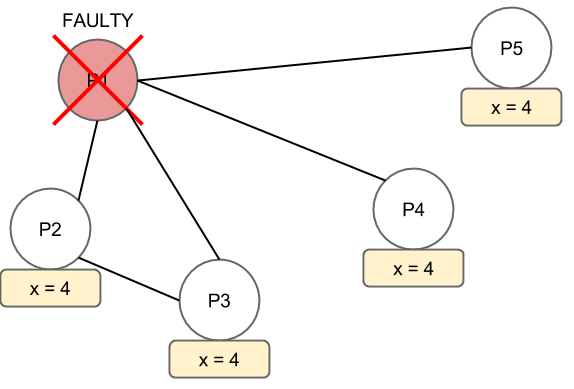
\includegraphics[width=0.5\textwidth]{consensus}
	\caption{A distributed system consisting of a number of nodes with a faulty one.}
	\label{consensus}
\end{figure}

The fundamental problem behind this, is that you cannot rely on the individual processes to be reliable and thus solely store the value. This means, that every process should store this value and should be able to be altered somehow. This boils down to a well-known problem - The Two Generals Problem.

% Måske burde the two generals problem komme her?

% Enig, har sat det ind her i stedet for.

\subsection{Motivation}
The elements of the problem presented serve as motivation behind consensus in a system of unreliable components. Because how do you know for certain what a value is, when you for sure know that some components must be faulty at some point?

\subsubsection{The Two Generals Problem}
The basic problem of reaching consensus in a distributed network can be illustrated by the Two Generals Problem analogy.

\begin{figure}[h]
	\centering
	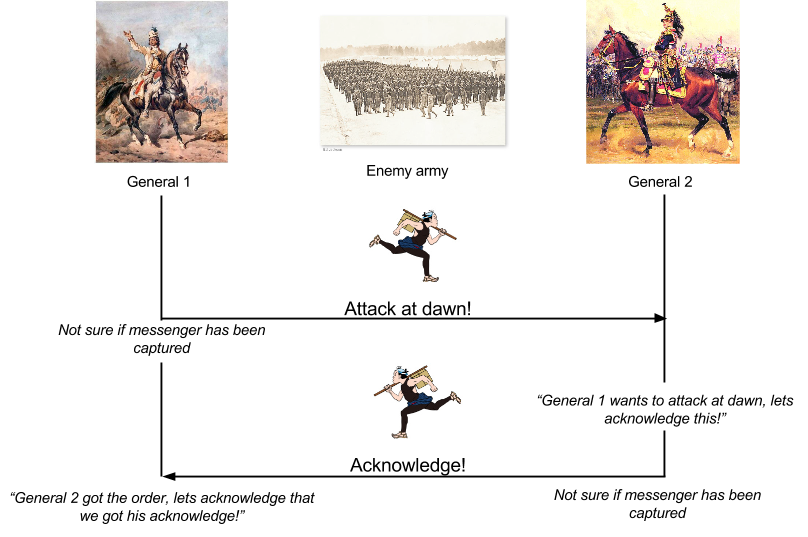
\includegraphics[width=0.8\textwidth]{twogenerals}
	\caption{Two generals tries to agree on when to attack the enemy by sending a messenger, but they are not sure the messenger survives his trip between their camps.}
	\label{generals}
\end{figure}

In the figure\ref{generals} below we see two generals of the same army who want to attack an enemy army. But they have to attack at the same time in order to win. They cannot communicate directly to each other since they are at different fronts of the battlefield i.e. in their own camps. In the context of a distributed system, the generals here can be seen as two processes trying to agree on a value.
General 1 then sends out a messenger to tell the second general, that they should attack at dawn. The second general then receives this message, but the first general cannot be sure of this (the messenger might be captured or killed by the enemy on his way to the second general and vice versa). Again, in the context of distributed system, the unreliability of messenger can directly related back to the unreliability of message transmission in a normal distributed system. In terms of Byzantine failure, this can be illustrated by the messenger being captured by the enemy and turned to spy on the generals i.e. given false information.
So the second general sends the messenger back in order to acknowledge this. But the first general also has to acknowledge this, resulting in a never ending run for the poor messenger - thus the generals can never agree on when to attack the enemy.

\subsubsection{Properties of distributed consensus}
When want to define consensus, the goal is to satisfy a set of requirements i.e. properties that the distributed system must uphold. These are used to describe the systems fault tolerant features related to faulty processes. A faulty process can either fail by crashing or experience a Byzantine failure. Such a failure in the context of distributes system occur when e.g. a process for some reason transmits incorrect or malicious data throughout the network. Due to the arbitrary results of these kinds of failures, properties of a system are often distinguished by either tolerating them or not. A main difference in terms of properties of a system whether it tolerates Byzantine failures or not, is the validity and integrity. The integrity property for a system that does not tolerate Byzantine failures is as following\cite{DistributedSystems}.

\begin{itemize}
\item non-Byzantine failure tolerant:
	\begin{itemize}
	\item \textbf{Validity}: If all processes propose the same value \textit{v}, then all correct processes decide \textit{v}.
	\item \textbf{Integrity}: Every correct process decides at most one value, and if it decides some value \textit{v}, then \textit{v} must have been proposed by some process.
	\end{itemize}
\item Byzantine failure tolerant:
	\begin{itemize}
	\item \textbf{Validity}: If all correct processes propose the same value \textit{v}, then all correct processes decide \textit{v}.
	\item \textbf{Integrity}: If a correct process decides \textit{v}, then \textit{v} must have been proposed by some correct process.
	\end{itemize}
\end{itemize}

The clearest commonality here, is that you should always be able to say that all correct processes must be able to decide on the same value or state, as mentioned earlier. Though the main difference is that with Byzantine processes, you must be able to say if they are all correct before stating they can derive the same value. This fact differentiates many solutions to this problem, depending on which property set they can satisfy. \\
Also, as discussed in \cite{Raft} a consensus algorithm for a non-Byzantine system has the following properties: safety, availability, timing interdependency, and majority vote on procedure calls. The safety property can be directly related back to our validity and integrity properties, as the system's safety and availability is measured be the correctness of return result upon a request.

% section introduction (end)

\section{Raft}
\label{sec:raft}
As of writing this report, the most recent proposal to solving the consensus problem is Raft~\cite{Raft}. Diego Ongaro and John Oustershout argue that most consensus algorithms, such as Paxos~\cite{Paxos} suffer from poor understandability and are hard to understand and implement. Diego and John introduce Raft as a simple and understandable solution to the consensus problem.

\subsection{Components of Raft}
Raft is described as having three main components, where the first two describes the behaviour of algorithm and the last describes how the algorithm ensures consensus safety properties.

\begin{itemize}
  \item \textbf{Leader election}: A strong leader is elected which responsible for keeping the rest of the system in consensus for a term that ends if it fails.
  \item \textbf{Log replication}: The leader must accept log entries from clients and replicate them across the cluster, forcing the other servers to agree with its own log~\cite{Raft}.
  \item \textbf{Safety}: The specified design provides safety such that\cite{Raft}:
      \begin{itemize}
        \item \textbf{Election Safety}: There is always at most one leader in the system.
        \item \textbf{Leader Append-Only}: A leader can only append new entries to its log i.e. it cannot overwrite existing entries.
        \item \textbf{Log Matching}: The logs of all servers are matching up to their latest common index and term.
        \item \textbf{Leader Completeness}: No newly elected leaders will overwrite other server's log if its own log entry is not up to date.
        \item \textbf{State Machine Safety}: When a server updates its log it must be up to date with the leader's log.
      \end{itemize}
\end{itemize}

% TODO: Maybe rewrite below to fit new chapter

The above description of Raft serves as a rough overview of the algorithm. A more detailed description will be given during the implementation since the paper has implicit or unclear implementation specific components that we have to figure out ourselves. So as we every component is describes our experiences and findings in terms of implementation specific choices will thus be documented.

\section{Requirements} % (fold)
\label{sec:requirements}
The tool we are implementing should serve as an illustration tool to show how the Raft algorithm works for given scenarios of faulty processes in a distributed system.
The requirements are split into two different aspects i.e. functional and quality attributes:
\subsection{Functional requirements}
The end product must satisfy the following functional requirements given the MoSCoW method:
\begin{enumerate}
\item The tool must illustrate a scenario of a given set of processes in a distributed system, in which a leader is elected.
\item The tool must be an implementation of the Raft algorithm as specified in \cite{Raft}.
\item The user should be able to input parameters to vary the scenario, such as the number of processes.
\item The user must then be able to disconnect any process.
	\begin{enumerate}
	\item If a leader is disconnected a new leader must be elected automatically.
	\end{enumerate}
\item The user must be able to request that a log entry is replicated to the system at run time.
\item The tool could be further extended with a visualisation of the given distributed system.
\end{enumerate}
\subsection{Quality requirements}
The quality requirements of the illustration tool are inherited from the properties that are provided by the Raft algorithm.
	\begin{enumerate}
	\item The Raft implementation should have the following properties: Safety, availability, timing independence, and that commands complete as soon as a majority has responded.
		\begin{enumerate}
		\item Safety: The properties described in section \ref{sec:raft} about Raft.
		\item Availability: The system should be available as long it is possible to elect a leader through a majority vote.
		\item Timing independence: Safety should not depend on the timing of the system, i.e. the speed of a given process should provide it with an advantage in terms of the consensus of the system. For this, it is specified that:
		\begin{center}
		$broadcastTime << electionTimeout << MTBF$ \cite{Raft}.
		\end{center}
		\end{enumerate}
	\end{enumerate}
% section requirements (end)

\section{Analysis} % (fold)
\label{sec:analysis}

In this section we will analyze and describe our approach on implementing Raft with relation to the purpose of this project and with relation to achieve a more fault-tolerant and robust implementation.

\subsection{Existing Raft Implementations} % (fold)
\label{sub:existing_raft_implementations}

The application of consensus algorithms such as Raft is many, but the most generic applications are databases and service discovery systems. As Raft mostly fits applications in the low level end of the stack, it will also be best suited to be implemented in a more low level and light language such as C, C++ or Go. Erlang would also be a great fit with its fault-tolerant features.

Raft have already been implemented in several versions and in many languages. Diego Ongaro himself has implemented Raft in C++ (LogCabin\footnote{https://github.com/logcabin/logcabin}), CoreOS\footnote{A new Linux operation system fork made for server deployments.} uses etcd\footnote{https://github.com/coreos/etcd}, which is a Raft implementation in Go used for service discovery.

If a Raft implementation was needed for real usage, the solution would have been to extend some of the rich open source implementations already available in solid languages as Go and C. But as mentioned in the introduction, the scope of this project is to learn about Raft with relation to fault-tolerance by implementing it. To be able to cover as much of Raft as possible in the time scope, that language chosen for implementation is JavaScript, because it would allow more productivity.

% subsection existing_raft_implementations (end)

\subsection{Testing} % (fold)
\label{sub:testing}

In order to be able to verify that the implementation satisfies the requirements and that to ensure a higher level of robustness, the software will be thoroughly tested. To document requirement satisfaction, the implementation will be black-box tested on the level of acceptance and integration.

In order to achieve robustness the implementation will also be white-box tested on the unit test level in order to test the behaviour of the different objects in situations and cases that are hard to foresee.

% subsection testing (end)

\subsection{Development Approach}
\label{sub:development_approach}

The approach used for implementing Raft has iterative with relation to the process. The Raft paper includes an informal specification~\cite[page~4]{Raft} with behaviour of the servers described by the state they are in or how to respond to requests. In order to have a more common language between the specification and the tests, the development approach Behaviour Driven Development (BDD)\footnote{Originally described by Dan North in the blog post http://dannorth.net/introducing-bdd/}~\cite{bddpaper}. The Behaviour Driven approach is iterative and have been used in the report with the following steps:

\begin{enumerate}
    \item Derive behaviour from the specification and write a failing test of the given behaviour.
    \item Write the simplest code that implements the behaviour and make the test pass.
    \item Refactor the code
    \item Repeat
\end{enumerate}

This is close to Test Driven Development, but with focus on writing tests that describes behaviour instead of testing methods as in unit tests.
One important aspect to make this approach work well is to derive the behaviour that seem most easy to implement first.

To facilitate writing tests with a BDD-aproach, the node-libraries \href{http://chaijs.com/}{\tt chai} together with \href{http://mochajs.org}{\tt mocha} 
% subsection our_approach (end)

% section analysis (end)

\section{Leader Election} % (fold)
\label{sec:leader_election}
In this section we will describe the component of leader election in Raft followed by a discussion of the design and implementation choices made during implementation.

\subsection{Leader election in Raft}
As mentioned in section \ref{sec:raft} one of the two main components of Raft is its leader election. After a successful leader election the given leader is responsible of replicating commands it receives from a client to the rest of the followers, which is explained in the log replication section \ref{sec:log_replication}. All servers contain an implementation of Raft, having a log of commands requested by clients. A server can be in three states: ``leader'', ``candidate'' or ``follower''. The servers convert to different states in different scenarious defined by the Raft specification and illustrated in figure~\ref{fig:state_state_machine}. As default the servers in the system will be in the ``follower'' state in which they act as an active part receiving heartbeat messages from the current leader. At most one leader exists at any given election term. The election term is incremented each time a new leader is elected. In distributed systems the term is the systems logical clock in which any entry in the server's log has a term attached to it in order to know when that value has been replicated to.

\begin{figure}[ht!]
\centering
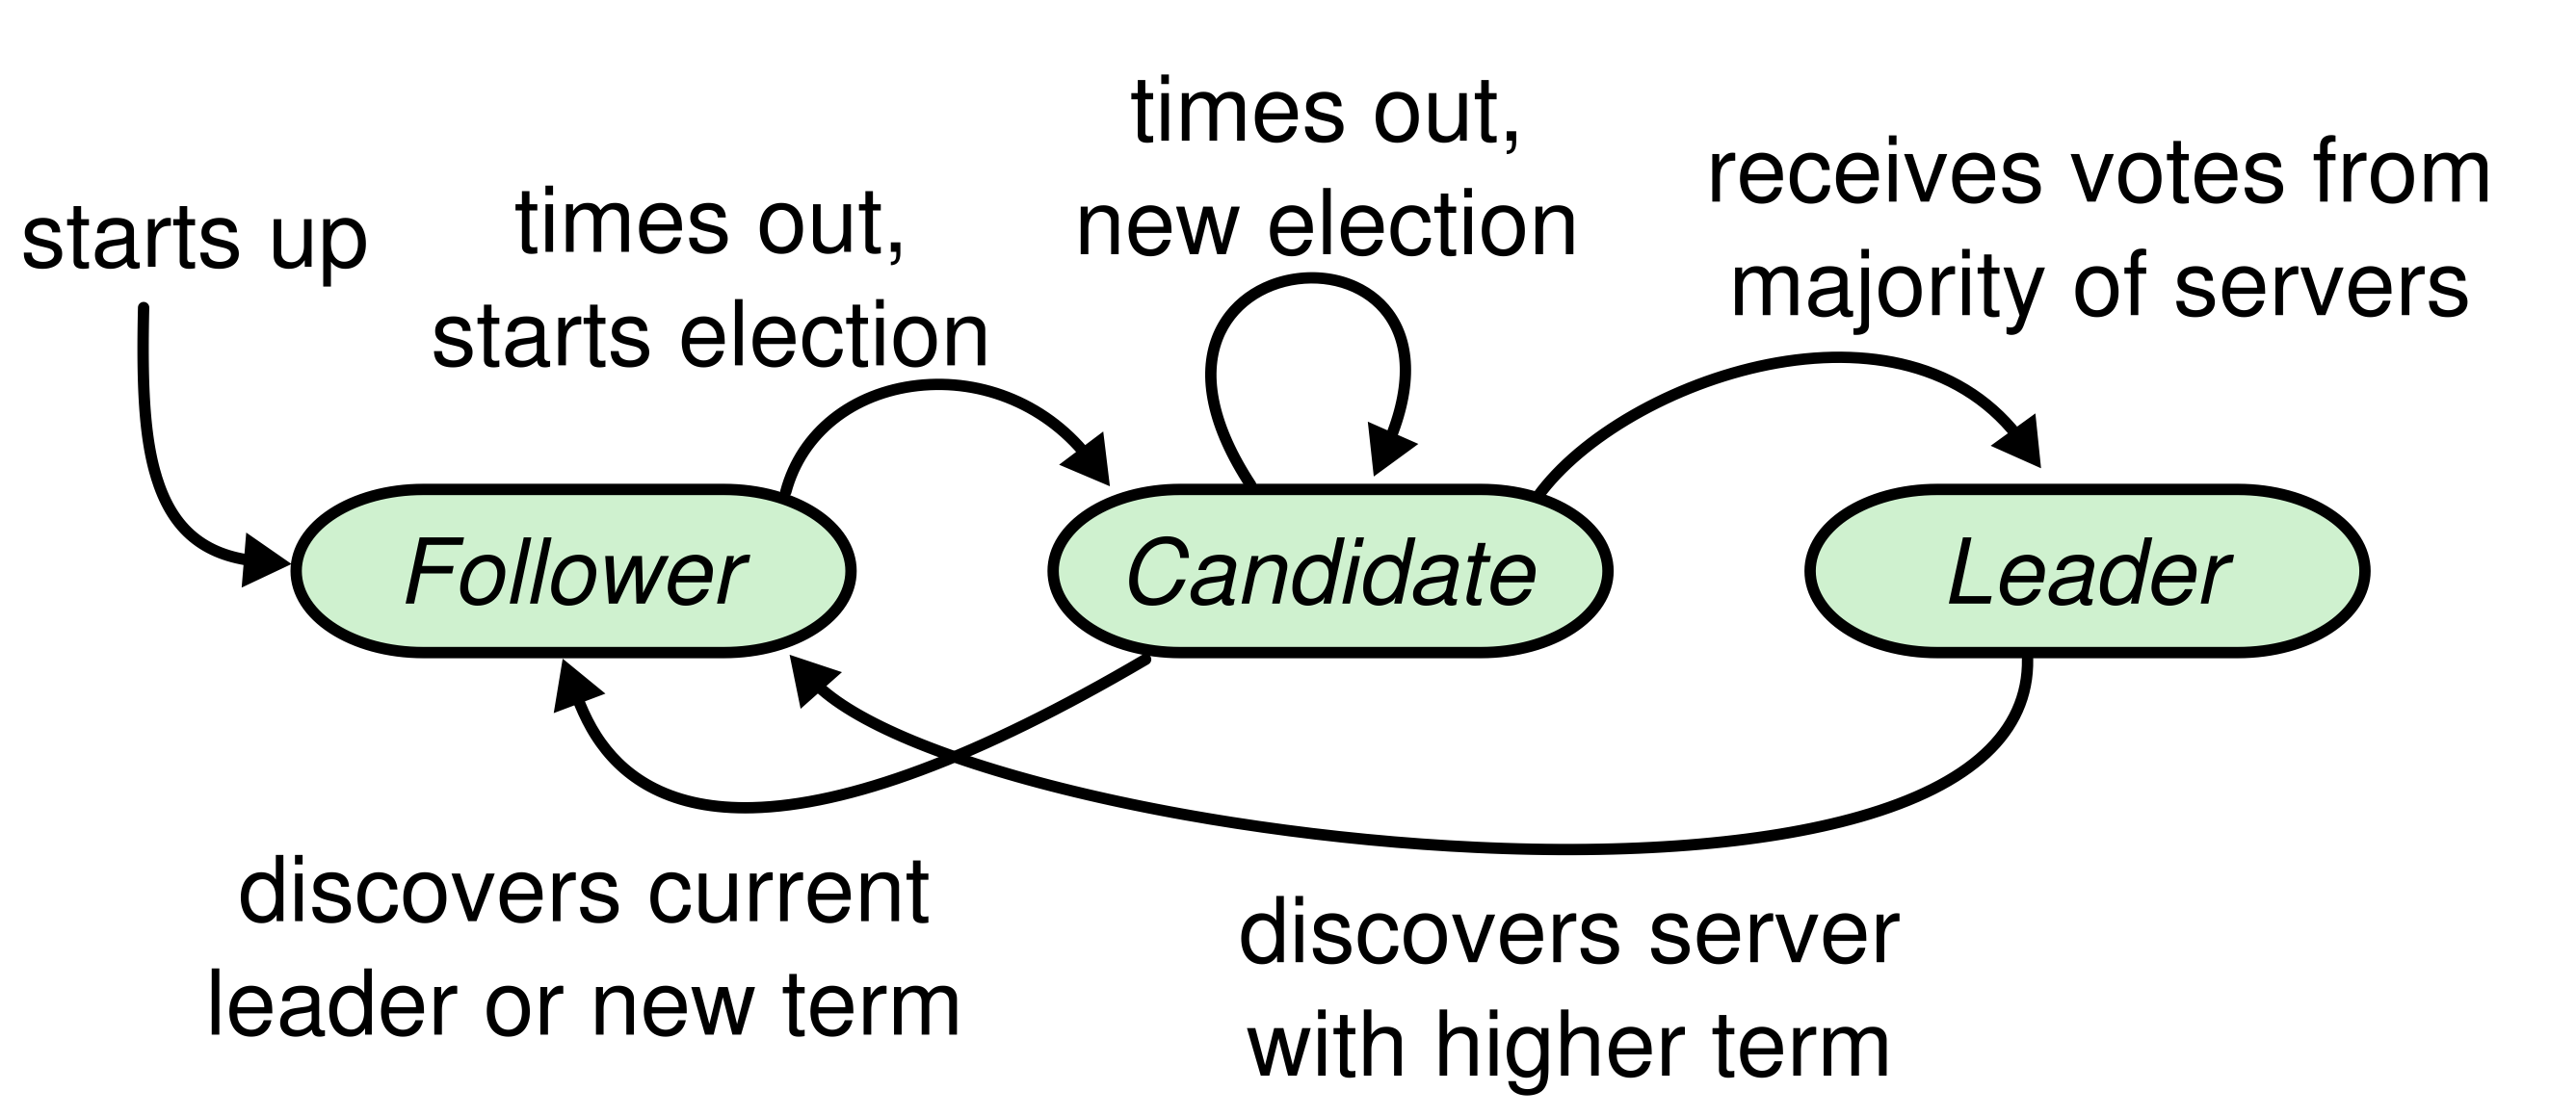
\includegraphics[width=0.6\linewidth]{figures/server_state_machine.png}
\caption{A graph illustrating the three different states of Raft servers and the situations in which they convert to other states. Figure taken from the Raft paper~\cite{Raft}.}
\label{fig:state_state_machine}
\end{figure}

Figure~\ref{fig:election_example} illustrates the scenario in which a leader is elected:

In the beginning of the illustration, on initial system startup, every server is a follower until $P1$ times out, because it has not received any valid heart beat messages from a leader. When $P1$ times out it becomes a ``candidate''. If this candidate receives a majority of votes it transitions to the leader state after which it has the responsibilities of a leader as described in section \ref{sec:raft}. The leader claims its leadership by sending out heartbeats, where if a server receives a heartbeat request from another server it is instantly converted to follower and recognizes the source as leader.

\begin{figure}[ht!]
\centering
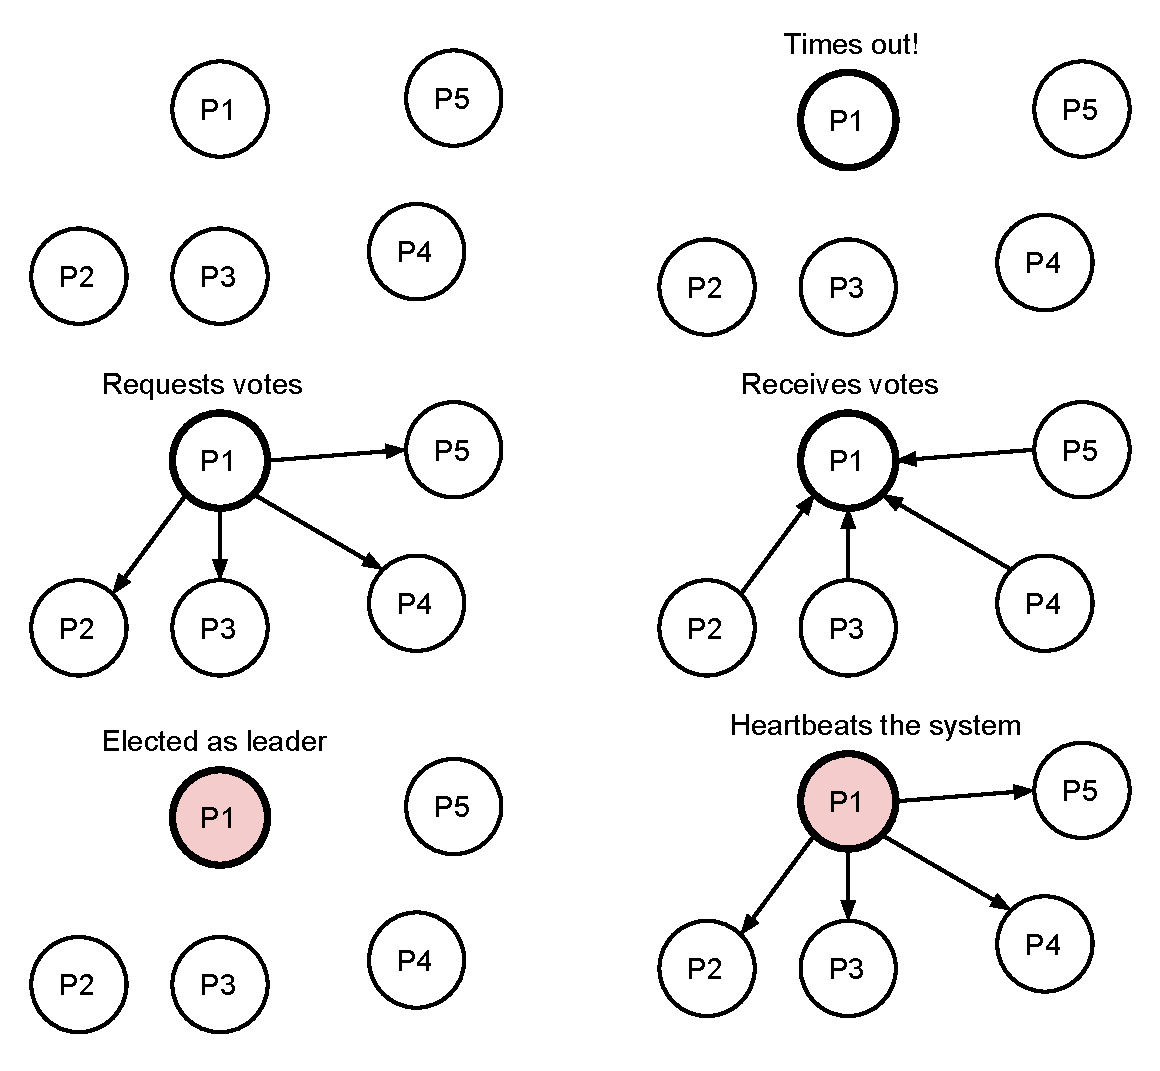
\includegraphics[scale = 0.5]{election-example}
\caption{A simple scenario where 5 servers are to obtain consensus by first electing a leader.}
\label{fig:election_example}
\end{figure}

Figure~\ref{fig:failure_example} shows how Raft will tolerate a faulty leader. Here we see that the leader $P1$ fails by crashing. $P4$ then times outs and initiates a new election.

\begin{figure}[ht!]
\centering
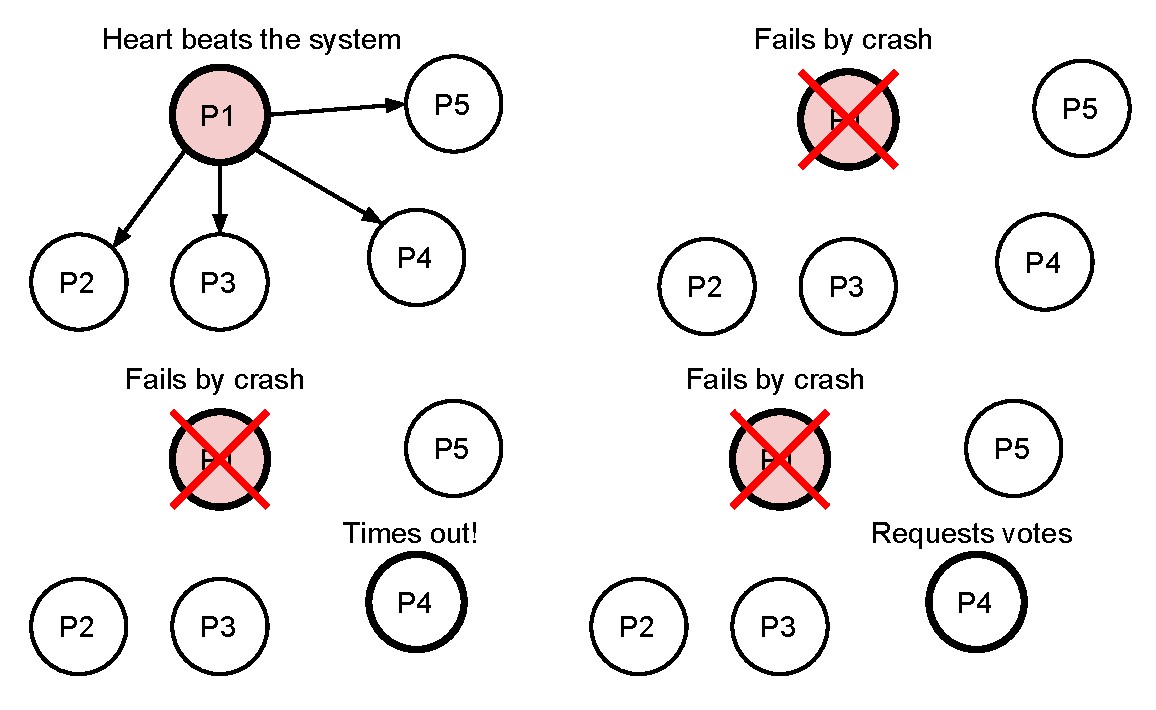
\includegraphics[scale = 0.5]{failure-example.pdf}
\caption{A simple scenario where a leader $P1$ crashes after which $P4$ times out and start a new election.}
\label{fig:failure_example}
\end{figure}

It should also be noted that upon transitioning to the candidate state and requesting votes, another server might have been requesting votes before this. In this situation the candidate would receive a heartbeat message from a leader with a term at least as large as its own, after which is transitions back to follower.
The situation in which a majority vote is not achieved by any candidate, the candidates will issue yet another election once they time out again. In order to avoid tied election such as these Raft uses a randomized time out within a given interval.

It should also be noted that since the availability, provided by Raft, relies on the majority votes and only non-Byzantine failures, the algorithm can thus only uphold these properties in a network where $3F \leq N$, where $F$ is the amount of failures and $N$ is the amount of processes in the system.~\cite{Fischer}

Looking back at the Two Generals Problem, Raft is only able to solve the problem if a majority vote would be possible which cannot be the case with only two ``servers'' (or generals). In order to solve this problem when utilising Raft, one must add another general to the scenario such that there are more than two servers in the system. We should also modify the problem such that the messenger always tells the truth (i.e. cannot suffer from Byzantine failures). Now that we have three generals and an ``uncapturable'' messenger, they will reach consensus by finding a leader after which he decides when to launch the attack.

% TODO: explain figure of different states (maybe take it from the Raft Paper)

% subsection leader_election_in_raft (end)

\subsection{Implementation} % (fold)
\label{sub:leader_election_implementation}

Our Raft implementation consists of two major parts:

\begin{enumerate}
  \item An election timer that is reset with a random time in a specified interval
  \item RequestVote RPC implementation with methods for handling invocation and receiving RequestVote RPC request and response
\end{enumerate}

\subsubsection{Election Timer} % (fold)
\label{ssub:election_timer}

The election timer is implemented by keeping state of the amount of milliseconds left and decrement this value every millisecond using the JavaScript function \verb$setInterval$. The timer is then reset in five situations:

\begin{itemize}
  \item On initialization
  \item On restart
  \item When receiving an AppendEntries RPC
  \item When it has started an election
  \item When it has voted for another candidate
\end{itemize}

% subsubsection election_timer (end)

\subsection{RequestVote RPC} % (fold)
\label{sub:requestvote_rpc}

If the election timer reaches zero it will start an election by sending a Remote Producure Call (RPC) request called \emph{RequestVote RPC}, where each server responds whether or not it will grant a vote to the candidate. As the votes are independent to each server they can be sent out in parallel as specified in the Raft paper. Since our implementation is a simulation with objects instead of processes or servers and JavaScript does not have threads, it is not possible to do true parallel computing. But since it is a simulation, we simulate parallel requests with the JavaSript method \verb$setTimeout$, which delays the execution of a given function. To make the simulation more like real requests, they are delayed given by a random amount of milliseconds in a given interval.

This implementation is fine for the visualization, but since we also want to verify the implementation through tests, it is not convenient to make the election random since you cannot assert a random election result. It would be possible to assert a given property such as ``assertion that there is at most one leader after x seconds''. Although this could be a viable test it is not convinient either, since it will make the tests slow and thereby slow down the development flow.

In order to easily test the execution of the RequestVoteRPC, we have made a protocol for communicating between servers in Raft. The protocol is an object that delegates a method call to a target and is injectable in the Server object. The delayed implementation explained above is seen in the protocol object \verb$DirectAsync$. The protocol used in testing will call methods directly on the target object and is called \verb$Direct$.

% subsection requestvote_rpc (end)

% - Problems
%   - Intro:
%     - Random election timer
%     - Parallel RPC's (RequestVote)
%     -
%   - Raft uses a randomly initiated timeout to do election:
%     - Every follower has an election timer given by a random time interval that
%       is reset with a new random time given by a random interval between t_1 and t_2.
%   - Problem:
%     - Hard to test, because:
%       a. you cannot assert a random result.
%       b. you do not want tests to be dependent on a time interval, because then you have slow tests
%       c. you cannot guarantee any test will pass every time if it is random (every test run is different)
%   -
%
% subsection implementation (end)

% section leader_election (end)

\section{Log Replication} % (fold)
\label{sec:log_replication}

In this section we will describe how Raft handles log replication, discuss some of the design decisions we have taken within Raft and describe the challenges with the implementation.

\subsection{Log Replication in Raft} % (fold)
\label{sub:log_replication_in_raft}

The general purpose of the log replication feature in a consensus algorithm and in Raft is to keep a log history of commands applied to the state machine in order to compare integrity between servers.

Log entries are appended to the log when a client requests a given command to be applied. The flow of receiving the request from the client, commiting the command to the log and responding the client is illustrated in figure~\ref{fig:log_replication_example}. In overall the steps of committing a command in Raft can be written as:

\begin{enumerate}
  \item Client sends request to the leader with command
  \item Leader appends command to own log
  \item Leader replicates log to followers in parallel
  \item When the command is replicated and commited to a majority of the servers in the cluster, the leader will respond positively to the client and apply the command to the state machine. \label{enum:client_request_final}

\end{enumerate}

\begin{figure}[ht!]
  \centering
  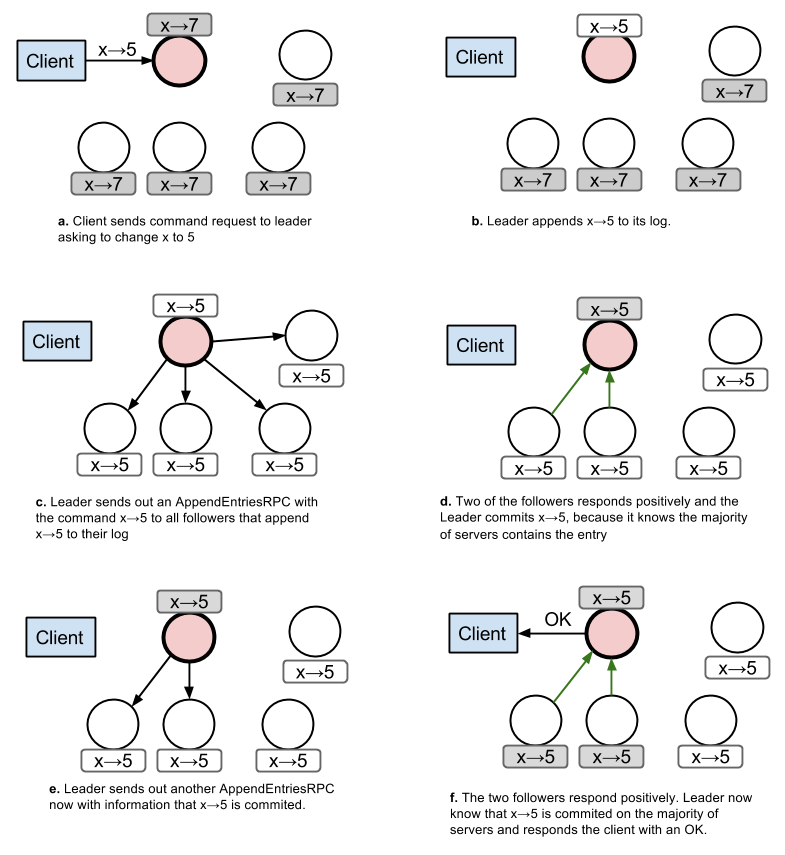
\includegraphics[width=0.7\textwidth]{figures/log-replication-example.png}
  \caption{An illustration of how the leader successfully applies a command from the client. At first \emph{(a)} the client requests the leader to apply the command x$\rightarrow$5 to the state machine, then \emph{(b)} it applies the command to its own log and \emph{(c)} replicates it to the followers. \emph{(d)} The followers respond positively if the command is applied to their log and the leader commits the entry from the client, when a majority of the servers have appended the log. \emph{(e)} The followers will receive information that the entry is commited and \emph{(f)} when the leader knows that a majority of the servers have applied the command, it will respond to the client positively and append it to the state machine}
  \label{fig:log_replication_example}
\end{figure}

% Maybe do not include this headerline
\subsubsection{AppendEntries RPC/Heartbeat} % (fold)
\label{ssub:appendentries_rpc_heartbeat}

The log replication mechanism explained in these steps are in Raft the same heartbeat mechanism used for claiming leadership as explained in section~\ref{sec:leader_election}. The hearbeat/log replication request is a Remote Procedure Call (RPC) called \emph{AppendEntries RPC}. The leader invokes the RPC with information for the follower duplicate the leaders log and be in consensus. The follower then responds the leader with success if it is fully replicated or else failure.

% subsubsection appendentries_rpc_heartbeat (end)

% Maybe do not include this headerline
\subsubsection{Commiting Log Entry} % (fold)
\label{ssub:commiting_log_entry}

The first time a server receives an AppendEntries RPC it will just append it to the log. A log entry is committed by the leader when the leader knows that a majority of the servers have appended the given log entry to their log. The log entry is then commited on a follower, when the leader sends out information (through \emph{AppendEntries RPC}) that the index of a given log entry is commited. The log entry is safe to apply to the state machine, when a majority of the servers have commited the entry.

% subsubsection commiting_log_entry (end)

\subsection{Handling Log Inconsistency} % (fold)
\label{sub:handling_log_inconsistency}

The scenario explained this far is the successful one, but in distributed systems failures such as network partitions and single server crashes are not rare and should be handled. Raft has behaviour for handling different kinds of log inconsistencies, which compared to the true log of the leader can be:

\begin{enumerate}
  \item A follower is missing entries
  \item A follower has extra entries
  \item A follower is both missing entries and has extra entries
\end{enumerate}

All situations of inconsistencies are handled by forcing the followers to duplicate the leaders log. The first situation is handled through the AppendEntries RPC by finding the largest common commited index and replicate the missing entries from the leader. The second scenario is handled by finding the largest common commited index and delete all entries following. Thereafter the situation is as the first and handled so. The last scenario is handled as the second.

% subsection handling_log_inconsistency (end)

\subsection{Implementation} % (fold)
\label{sub:log_replication_implementation}

The log and heartbeat are two implementation specific parts of the Raft algorithm that is not described in implementation details.

Normally the log should be persistent, but since the implementation in this project is only for visualization, persistency is not implemented. The log is implemented as an object \verb$Log$ that works as an abstraction on top of a simple array containing the entries. For a programmer this abstraction is important since Raft is documented and specified as being a 1-indexed system, where most databases and arrays in various programming languages are 0-indexed.

Besides replicating its log, the leader also need to keep state of the progress of the follower's logs. More precisely it need to know the next empty index of a given follower's log and the index of largest log entry that matches in the leader log. In our implementation this state is kept in the \verb$LeaderState$ object that is initialized (or reset) when a new leader is elected.

The heartbeat is implemented and used by the leader as an independent mechanism that sends an AppendEntriesRPC every $t$ milliseconds using the JavaScript function \verb$setInterval$. Alternatively the heartbeat could be dependent on the response of the follower by sending a heartbeat $i$ seconds after the leader got a response. But this would introduce extra complexity as we would need to handle the case where the follower is down.

The AppendEntriesRPC is as the RequestVoteRPC explained in section~\ref{sub:requestvote_rpc} done in parallel. In order to both be able to test the behaviour involing AppendEntriesRPC and simulate real requests in the simulation we have added AppendEntries to the \verb$Direct$ and \verb$DirectAsync$ protocols.

An important implementation detail of the log replication is that the log entries need to contain the index and the action of appending a log entry need to be idempotent as specified in the paper~\cite[p.~10]{Raft}. Our initial implementation was by using the array index of the log to control indexes, but this meant that if the delay of the RPC's was close to the heartbeat interval the leader would send two AppendEntriesRPC's to the same active follower without getting the result of the first AppendEntriesRPC which results in a race condition that makes the follower append the same entries twice. To avoid this the leader assigns an incremental index to the log entry when received by a client and secondly the method of appending a log entry is made idempotent. The code for the idempotent log append method is seen in code example~\ref{code:append_method}.

\lstinputlisting[label={code:append_method},caption={The method used by followers to append entries from the leader to the log. This method is idempotent, which means that appending the same entry to the exact same log twice (or more) will give the same result.}, language=JavaScript]{code_snippets/idempotent_append_entry.js}

% subsection implementation (end)

% section log_replication (end)

\section{Evaluation and Testing} % (fold)
\label{sec:evaluation_and_testing}
As mentioned in the analysis section\ref{sec:analysis} we are to evaluate our solution with white- and black box tests. Their description will thus be provided and followed by the results.

\subsection{White box tests}
The development of our solution was to iterate based on the behaviour of Raft. This included writing a test for each behaviour described in the condensed summary of Raft\cite{Raft}. For each of these tests its required functionality was then implemented in order to satisfy it.

%Forklar heraf resulterne af testene, og hvilke dele af koden der hører til hvilken 'behaviour'.

\subsubsection{Tests}
Although the functional tests, constructed during implementation, can be directly read in the code, a small example will be presented for completeness's sake.\\ \\
The following code snippet shows the test for the AppendEntries RPC attribute that a receiver should reply false if the given RPC call contains a term < currentTerm.
\lstinputlisting[caption=The test for the AppendEntries RPC Receiver implementation, language=JavaScript]{code_snippets/whitebox-test-example.js}

\subsubsection{Results}
The results for all of the whitebox tests can be seen in appendix~\ref{sec:results}.

\subsection{Black box test scenarios}
Verifying that our solution actually is an implementation of Raft requires more in-depth tests in the form of validating that we uphold the properties that are argued to provide consensus. This is done by constructing a set of scenarios that reflect the behaviour of the components of Raft: Leader Election, Log Replication, and Safety. The scenarios are as following with success criteria and a simple use case:

\subsubsection{Tests}

\begin{itemize}
\item \textbf{Leader Election}:
    \begin{enumerate}
    \item A leader is elected upon initiate start up of the system.
        \begin{enumerate}
        \item The user starts the program.
        \item Server $S$ times out.
        \item $S$ converts to candidate.
        \item $S$ receives a majority vote and converts to leader.
        \end{enumerate}
    \item A new leader must be elected if the current leader fails.
        \begin{enumerate}
        \item The user starts the program.
        \item A server $L$ is elected as leader.
        \item The user crashes $L$ at run-time.
        \item Server $S$ times out and starts a new election.
        \end{enumerate}
    \end{enumerate}
\item \textbf{Log Replication}:
    \begin{enumerate}
    \item Log entry is replicated through the system.
        \begin{enumerate}
        \item The user starts the program.
        \item A server $L$ is elected as leader.
        \item The user requests that a value $x$ is replicated.
        \item $L$ replicates $x$ such that each log of each server contains $x$ in their log at the correct term and index.
        \end{enumerate}
    \item Awoken follower get its log updated.
        \begin{enumerate}
        \item The user starts the program.
        \item A server $L$ is elected as leader.
        \item The user crashes a server $S$.
        \item The user requests that a value $y$ is replicated.
        \item The user wakes up $S$.
        \item $L$ updates $S$'s log such that it contains $y$ in its log at the correct index and term.
        \end{enumerate}
    \end{enumerate}
\item \textbf{Safety}:
    \begin{enumerate}
    \item There is at most one leader at any given term.
        \begin{enumerate}
        \item The user starts the program in which two servers $S_1$ and $S_2$ have the same election time out.
        \item A leader $L$, being the only one with an election time out smaller than both $S_1$ and $S_2$'s, gets elected.
        \item The user crashes $L$.
        \item Both $S_1$ and $S_2$ start their elections.
        \item Either $S_1$ or $S_2$ is elected as the new leader.
        \end{enumerate}
    \item Leader never overwrites its own log but only appends on to it.
        \begin{enumerate}
        \item The user starts the program.
        \item A server $L$ is elected as leader.
        \item The user requests that a value $x$ is replicated.
        \item The user requests that a value $y$ is replicated.%Er ikke sikker på at det illustrerer det korrekt.
        \end{enumerate}
    \item Logs of every server match each other up to their latest common index in their logs.
        \begin{enumerate}
        \item The user starts the program.
        \item A server $L$ is eleced as leader.
        \item The user requests that a value $x$ is replicated.
        \item The user crashes a server $S$.
        \item The user requests that a value $y$ is replicated.
        \item All the servers have a commonality that they know of $x$ but not $y$.
        \end{enumerate}
    \item The log of a leader contains all previous log entries of leader of previous terms.
        \begin{enumerate}
        \item The user starts the program with a server $L$ with the lowest election time out and $S$ with the second lowest.
        \item $L$ is elected as leader.
        \item The user crashes a server $S$.
        \item The user requests that a value $x$ is replicated.
        \item The user wakes up $S$
        \item The user crashes $L$
        \item $S$ has an up to date log.
        \end{enumerate}
    \end{enumerate}
\end{itemize}
Please note that there is no acceptance test for state machine safety. This is because there's is no actual state machine in our implementation, thus testing this would be impossible. Further details about this in section~\ref{sec:discussion}.

And referring back to requirements in section \ref{sec:requirements}. The solution should also satisfy the requirements about availability and timing independence. The success criteria and scenarios for these requirements are as following:
\begin{itemize}
\item \textbf{Availability}:
    \begin{enumerate}
    \item As long as a majority vote is possible, a leader must always be elected. If not the system should become unavailable.
        \begin{enumerate}
        \item The user starts the program with five servers.
        \item A server $L$ is elected as leader.
        \item The user crashes $L$ and another server.
        \item A new leader $L'$ is elected as leader.
        \item The user crashes $L'$.
        \item The system becomes unavailable.
        \end{enumerate}
    \end{enumerate}
\end{itemize}
The last scenarios about safety, availability, and especially timing independence are hard to informally validate since the program simulates a concurrent system, in which the utilisation of a formal verification tool would be necessary, which is out of scope of this project. %TODO: ok?.

\subsubsection{Results}
The scenarios are implemented and test in the same way as done for the whitebox tests, in which we describe the each scenario with its underlying use case as the real test. Please refer to appendix TODO to see the results of these tests.
%Hvordan skal de præsenteres/dokumenteres?

    
% section evaluation_and_testing (end)

\section{Discussion} % (fold)
\label{sec:discussion}

% - Hvordan gik det?
% - Hvad var svært?
% - Hvad kunne vi gøre bedre?
% - Future improvements?

% section discussion (end)

\section{Conclusion} % (fold)
\label{sec:conclusion}

% section conclusion (end)


\bibliography{references}{}
\bibliographystyle{plain}

\appendix
\section{Results}
\label{sec:results}
\begin{small}
\begin{spverbatim}


  Rules for Followers
    Respond to RPCs from candidates and leaders
      ✓ responds to RequestVote RPCs from candidate (88ms)
      ✓ responds to AppendEntries RPC from leader 

  Rules for Candidates
    On conversion to candidate, start election:
      ✓ increments currentTerm 
      ✓ votes for self 
      ✓ resets election timer 
      sending RequestVote RPCs to all other servers
        ✓ is granted a vote 
        ✓ is not granted a vote if vote term is less than target server's term 
        ✓ is converted to follower and updates term when outdated 
        ✓ is not granted a vote when target server that has already voted for another server 
        ✓ is not granted a vote when the candidate log is not up to date 
    If votes received from majority of servers, become leader
      with 5 peers in network
        ✓ becomes leader when receiving 3 votes 
        ✓ does not become leader when receiving 2 votes 
      with 4 peers in network
        ✓ becomes leader when receiving 3 votes 
        ✓ does not become leader when only receiving 2 votes 
    If AppendEntries RPC received from new leader: convert to follower
      ✓ becomes follower when receiving AppendEntries from leader 
    Receiver AppendEntries Implementation
      ✓ replies false if term < currentTerm 
      ✓ replies true if term >= currentTerm 
      ✓ reply false if log doesn't contain entry at prevLogIndex 
      ✓ reply false if log doesn't contain entry at prevLogIndex whose terms matches prevLogTerm 
      ✓ reply true if log does contain entry at prevLogIndex whose terms matches prevLogTerm 
      ✓ appends any new entries not already in the log 
      ✓ sets commitIndex=leaderCommit if leaderCommit > commitIndex and leaderCommit < index of last new entry 
      ✓ sets commitIndex=index of last new entry if leaderCommit > commitIndex and index of last new entry < leaderCommit 
      ✓ sets commitIndex=leaderCommit of last new entry if leaderCommit > commitIndex and index of last new entry == leaderCommit 
      If an existing entry conflicts with a new one
        ✓ deletes existing entry and all that follows 

  Client Log Entry Request
    ✓ client sends log request to server 
    ✓ client sends log request to a follower 

  General rules for servers
    ✓ If successful: ipdate nextIndex and matchIndex for follower. 
    ✓ If AppendEntries fails because of log inconsistency: decrement nextIndex and retry. 
    If there exists an N such that N > commitIndex .... (advance commit index)
      ✓ updates commitIndex if majority of servers matches that index 
      ✓ does not update commitIndex if majority of servers does not match that index 


  31 passing (120ms)


\end{spverbatim}
\end{small}


\end{document}
